\chapter{Hashing and dictionaries}

Dictionaries are abstract data types that support insertions and
memberships. One way in which dictionaries are implemented are using hash
tables. Even beyond dictionaries, hashing and hash tables have a lot of
applications in computer science. In the lectures so far, we have seen hash
functions that are completely random. These are not always practical for the
following reason.

Let us say that we have a universe $U$ and a set
$S \subseteq U$ such that $|S| \ll |U|$, that we want to
store and do membership on. Let us assume that $|S| = m$ and
$|U|=n$. Ideally we want the data structure to use space proportional
to the size of the set $S$. We saw from the maximum load of the balls-in-bins
process that if we choose a random function $h:U \to [m]$, then with
high probability, the maximum load is only $\Theta(\log n/\log\log n)$. But,
what this hides is the fact that if we were to a random function $h$, then we
need $n\log m$-space to store the hash function itself. For doing membership, we
need an efficient way to compute the value $h(x)$ for any $x$. But then, this
defeats the whole purpose of this exercise - we could have as well used an
$O(n)$-bit array to store the set $S$!

In the rest of this chapter, we will look at how to design data structures for
\emph{static} and \emph{dynamic} dictionaries using limited independence.

\section{Universal hash families}

One important class of hash functions that are simple to construct and evaluate
while still giving good guarantees for the dictionary problem are the universal
hash families, that were initially studied by Carter and Wegman.

\begin{definition}
  Let $U$ be a universe of size $n$, and $S$ a set of size $m$. A family of hash
  functions $\mathcal{H}$ is said to be $k$-universal if for any elements
  $x_1, x_2, \ldots, x_k$, we have
  \begin{align*}
    \Pr_{h \sim \mathcal{H}} \left[h(x_1) = h(x_2) = \cdots = h(x_k) \right] \leq \frac{1}{n^{k-1}}.
  \end{align*}

  \marginnote{A family of strongly $k$-universal hash functions is also known as
    a $k$-wise independent hash family.}  The family $\mathcal{H}$ is said to be
  \emph{strongly} $k$-universal if for any elements $x_1, x_2, \ldots, x_n$ and
  values $y_1, y_2, \ldots, y_n$, we have
  \begin{align*}
    \Pr_{h\sim \mathcal{H}}\left[\bigcap_{i=1}^k (h(x_i) = y_i) \right] = \frac{1}{n^k}.
  \end{align*}
  \label{defn:univ-hash}
\end{definition}

The nice thing about universal hash families are that there are even
\emph{explicit} $2$-universal hash families that have only a few number of
functions (and hence can be represented and evaluated efficiently) and which
satisfy weaker forms of the bounds that we saw earlier, that make them amenable
to being used in practice. Before we see constructions of such hash families,
let us go back to computing the maximum load in the balls-in-bins process, but
now using $2$-universal hash families.

Consider the following version of the balls-in-bins process: there are $n$ balls
and $n$ bins. You choose a function $h$ uniformly at random from a $2$-universal
hash family $\mathcal{H}$. Now for each $i$, we place ball $i$ in bin $h(i)$. We
want to find out the maximum load on any bin when we do this process.

Let $X_{ij}$ denote the indicator random variable that denotes whether balls $i$
and $j$ land up in the same bin. Since $h$ is $2$-universal,
$\Pr[X_{ij}=1] \leq 1/n$. The total number of collisions is given by
$X = \sum_{i<j} X_{ij}$, and therefore
$\E[X] \leq \binom{n}{2}\frac{1}{n} \leq \frac{n}{2}$. Using Markov's
inequality, we can say that $\Pr[X \geq n] \leq 1/2$. If the maximum load is
$Y$, then clearly $\binom{Y}{2} \leq X$. Therefore,
$\Pr[\binom{Y}{2} \geq n] \leq 1/2$, and this shows that
$\Pr[Y \geq 1 + \sqrt{2n}] \leq 1/2$. While this is nowhere as good as the bound
in the truly random case, we will see how this will be useful when we analyze
perfect hashing.

\subsection{Dynamic dictionaries using $2$-universal families}

Suppose we want to perform membership queries on a dynamic set that is modified
by insertions and deletions. A data structure that supports the insert, delete
and search operations is called a dynamic dictionary and we will now see how
$2$-universal hash families provide expected constant time per operation.

Let us say that we have a sequence of $r$ requests, of which there are $n$
inserts. The number of deletes are also upper-bounded by $n$, and $n \leq
r$. Let $U$ be the universe of elements.

\begin{lemma}
  Let $\mathcal{H}$ be a $2$-universal hash family of functions $h:U\to [n]$ for
  an integer $n$. For any $x\in U$, $S\subseteq U$, and $h\in \mathcal{H}$,
  define the number of collisions with $x$ as
  $$\textup{\coll}(x,S,h) = |\{y\in S ~|~ h(x) = h(y) \}|.$$ Then
  $$\E_{h \sim \mathcal{H}} [\textup{\coll}(x,S,h)] \leq |S|/n.$$
  \label{lem:dyn-dict-chain}
\end{lemma}
\begin{proof}
  We can write the expectation as follows.
  \begin{align*}
    \E_{h\sim\mathcal{H}}[\coll(x,S,h)] &= \sum_{h\in \mathcal{H}} \frac{\coll(x,S,h)}{|{\cal H}|}\\
    & = \frac{1}{|{\cal H}|} \sum_{h\in {\cal H}} \sum_{y\in S} \llbracket h(x) = h(y)\rrbracket  = \frac{1}{|{\cal H}|} \sum_{y\in S}\sum_{h\in {\cal H}} \llbracket h(x) = h(y)\rrbracket
  \end{align*}
  Since ${\cal H}$ is $2$-universal, we have $\Pr_{h\sim {\cal H}}[h(x) = h(y)] \leq 1/n$, and therefore, for any $x\neq y$ we have $|\{ h\in {\cal H} ~|~ h(x) = h(y)\}| \leq |{\cal H}|/n$. Thus we can rewrite the earlier equation as
  \begin{align*}
    \E_{h\sim\mathcal{H}}[\coll(x,S,h)] &= \frac{1}{|{\cal H}|} \sum_{y\in S}\sum_{h\in {\cal H}} \llbracket h(x) = h(y)\rrbracket \leq \frac{1}{|{\cal H}|} \sum_{y\in S} \frac{|{\cal H}|}{n}\\
    &= \frac{|S|}{n}.
  \end{align*}
\end{proof}

This lemma suggests the following method for storing the dictionary. Construct a
$2$-universal hash family ${\cal H}$, and choose a hash function $h\in {\cal H}$
uniformly at random. For a sequence of requests, insert and delete using the
hash function $h$. The time of insertion, deletion and searching is bounded by
the length of the chain. From Lemma~\ref{lem:dyn-dict-chain}, we know that if we
choose $n$ to be larger than the total number of insertions that we perform,
then the expected size of the chain is at most $1$.
\begin{theorem}
  Let $t(h,r)$ be the time taken to respond to $r$ requests (including
  insertions, deletions and searches) when using a hash function
  $h\in {\cal H}$. Consider any sequence of $r$ requests that includes $s$
  insertions, and let ${\cal H}$ be a $2$-universal hash family of functions
  that map $U$ to $[n]$ where $n=O(s)$. Then the expected time for responding to
  all the $r$ requests is $\E_{h\in {\cal H}} [ t(h,r) ] = O(r)$.
  \label{thm:dy-dict-bound}
\end{theorem}

This follows almost directly from Lemma~\ref{lem:dyn-dict-chain}, assuming that
we can evaluate the hash function $h\in {\cal H}$ in $O(1)$-time since we know
that the length of the chain in the has table is $O(1)$ when $n > s$. The set of
all functions from $U$ to $[n]$ is a universal hash family, but they require
$|U|\log n$ bits to represent. Next we will see explicit $2$-universal hash
families that can be represented much more succinctly. All these constructions
naturally extend to $k$-universal families.

\subsection{Explicit constructions}

The first construction of a $2$-universal family was described by Carter and
Wegman. Let $U$ be a set of $m$ elements, and the hash table is of size $n$
where $n < m$. Let $p$ be a prime number at least as large as $m$. The family ${\cal H}$ is defined as follows:
\begin{align*}
  {\cal H} = &\{ h_{a,b} ~|~ 1\leq a \leq p-1, 0\leq b\leq p-1 \}, \text{ where }\\
  &h_{a,b}(x) = ((ax + b) (\rem p)) (\rem n).
\end{align*}

Notice that the number of functions in ${\cal H}$ is $\Theta(m^2)$ (as opposed
to $\Theta(n^m)$ when we use truly random functions). Sampling a uniformly
random function amounts to sampling two numbers ($a,b$), independently and
uniformly at random from $[p]$. Any function in the family can be represented
with $\Theta(\log m)$ bits, and the hash function $h_{a,b}$ can be computed
efficiently.

\begin{theorem}
  The family ${\cal H}$ given above is $2$-universal.
  \label{thm:2-univ}
\end{theorem}
\begin{proof}
  We want to show that for $x\neq y$,
  $\Pr_{a,b} [h_{a,b}(x) = h_{a,b}(y)] \leq 1/n$.

  Firstly, note that if $ax+b = ay+b (\rem p)$, then $a(x-y) = 0 (\rem
  p)$. Since $p$ is a prime, this is impossible unless $x=y$. Furthermore, for any
  $(z_1, z_2)\in [p]^2$, there exists exactly one pair $(a,b)$ such that
  $ax+b = z_1 (\rem p)$ and $ay+b=z_2 (\rem p)$. This is given by
  $a = (z_1 - z_2)(x-y)^{-1}$ where the addition and inverse is taken in the
  finite field $([p],+,\times)$, and $b =z_1 - ax$. Thus the probability that
  $h_{a,b}(x) = h_{a,b}(y)$ for randomly chosen $a$ and $b$ is same as the
  fraction of pairs $(z_1, z_2)\in [p]^2$ such that $z_1 = z_2 (\rem n)$.  Now
  once we fix $z_1 \in [p]$, then there are $p/n - 1$ other possibilities for
  $z_2$ ($z_2 = z_1 + kn$, for different values of $k$). Thus, we have
  \begin{align*}
    \Pr_{a,b} [h_{a,b}(x) = h_{a,b}(y)] = \frac{p(p/n - 1)}{p(p-1)}\leq \frac{1}{n}.
  \end{align*}
\end{proof}

We will now look at the construction of a strongly $2$-universal family of hash
functions. \marginnote{In fact many of the constructions of $2$-universal hash
  families actually yield strongly $2$-universal hash families.}  The
construction that we will see will be very similar to the construction of the
universal hash family that we saw above. For this construction, let us assume
that $|U| = 2^m$ and $|S| = 2^n$ where $m>n$. We will think of the set $U$ as
binary strings of length $m$, and also as a finite field of cardinality
$2^m$. Similarly for $S$. Finite fields of size $2^m$ can be thought of as
polynomials of degree $m-1$ over the field $\mathbb{F}_2$. Every element in $U$
is a binary string, and equivalently the string of coefficients of the poynomial
of degree $m-1$ over $\mathbb{F}_2$.

\section{Perfect hashing}

In this section we are interested in designing hashing schemes that allow
$O(1)$-time for searching in the worst case. If our universe $U$ has size
$m >> n$ where $n$ is the size of the dictionary that we are storing, then if
the hash table is of size $O(n)$, there cannot be a single hash function that
will work for all dictionaries $S$. Our goal is to construct a small family of
hash functions ${\cal H}$ such that for every set $S$, there is a function
$h\in {\cal H}$ such that $h$ has only $O(1)$ collisions on the set $S$.

\begin{definition}
  A family ${\cal H}$ of hash functions $h:[m]\to [n]$ is said to be a
  \emph{perfect hash family} if for every $S\subseteq [m]$ such that $|S|<n$,
  there exists an $h\in{\cal H}$ such that for every $x\neq y \in S$,
  $h(x) \neq h(y)$.
  \label{defn:perfect-hash}
\end{definition}

Clearly, if ${\cal H}$ is the set of all functions $h:[m]\to [n]$, then
${\cal H}$ is a perfect hash family. But, as before we want a small set
${\cal H}$ such that each function $h\in {\cal H}$ is compactly representable,
and the function $h$ is easy to calculate. For the static dictionary problem, we
would also require that given the set $S$, it is easy to find the function $h$
that is perfect for $S$. This would count towards the pre-processing time of the
data structure. Unfortunately, even if we discount the time required for
pre-processing, perfect hash families exist only for a very small range of
values.

\begin{lemma}
  Let $U$ be a universe of size $m$. If ${\cal H} = \{h:[m] \to [n] \}$ is a
  perfect hash family for sets $S$ of cardinality $n$, then
  $|{\cal H}| = 2^{\Omega(n)}$.
  \label{lem:ph-lb}
\end{lemma}
\begin{proof}
  Let $h$ be any hash function in ${\cal H}$. Let $m_i$ be the number of
  elements in $[m]$ that are mapped to $i\in [n]$ by $h$. Then for
  $\prod_{i=1}^n m_i$ sets $S\subseteq [n]$, $h$ is perfect for $S$. If
  ${\cal H}$ is a perfect hash family, this would mean that
  $|{\cal H}| \prod_{i=1}^n m_i \geq \binom{m}{n}$. Since
  $\sum_{i=1}^n m_i = m$, we can upper-bound
  $\prod_{i=1}^n m_i \leq \left( \frac{m}{n} \right)^n$. Thus, we can write
  \begin{align*}
    |{\cal H}| &\geq \left(\frac{n}{m} \right)^n \binom{m}{n} \\
    &= \left(\frac{n}{m} \right)^n \frac{\sqrt{2\pi m}\left(\frac{m}{e}\right)^m}{\sqrt{2\pi n} \left( \frac{n}{e} \right)^n \sqrt{2\pi(m-n)} \left( \frac{m-n}{e} \right)^{m-n}} \Theta(1),
  \end{align*}
  where the second line follows from Stirling's approximation. Simplifying this
  equation give $|{\cal H}| = 2^{\Omega(n)}$.
\end{proof}

What this means is that unless $m = 2^{\Omega{n}}$, the hash family will not
have a size polynomial in $m$ and hence will not be efficiently representable.
If we relax the notion of perfect hashing to have a multi-level hash table, then
it is possible to construct a data structure for static dictionaries that allows
$O(1)$-search time in the worst-case, uses $O(n)$ space and can be represented
efficiently. This is what we see next.

\subsection{FKS hashing} \marginnote{FKS are the initials for Michael Fredman, J\'{a}nos Koml\'{o}s, and Endre Szemer\'{e}di who were the first to describe this hashing method in 1984.}

The idea of FKS hashing is to have two levels of hash tables. The first hash
function maps to a position in the hash table. Now, all the elements that map to
a particular index in the hash table are stored in a secondary hash table. The
hash functions are chosen such that the number of collisions of the primary hash
functions is small, and the there are no collisions for the secondary hash
function. Given the set $S$, the hash functions that work for $S$ can be
computed efficiently as well. Furthermore, if $|S|=n$, then the total size of
the data structure is $O(n)$.

We start with the observation that we saw earlier in this chapter. If we use a
hash table of size $n$ to hash $n$ items using a $2$-universal hash family, then
if $X$ is the number of collisions among the items, we can say that
$\Pr[X > n] \leq 1/2$. This means that given a set $S$, there is a function
$h\in {\cal H}$ such that the number of collisions given by $h$ on the set $S$
is at most $n$. We can find this function $h$, by sampling from ${\cal H}$
uniformly at random and counting the number of collisions. Since number of
collisions is at most $n$ with probability at least $1/2$, in expectation we
need to sample such $h$ at most twice.

Now, once we have such a function $h$, we will use secondary hash functions to
hash the elements that collide. If $c_i$ collisions happen for the $i^{th}$
entry of the primary hash table, we will use a $2$-universal hash family of
functions $h:[c_i] \to~[c_i^2]$. By the same calcalculation as before, the
number of collisions caused by this secondary hash function is at most $1$ with
probability at least $1/2$. Once again, we can find these hash functions if we
know the elements that collide due to the primary hash function $h$.

Finally, notice that the totally space required to store $S$ is the space to
store the $n+1$ hash functions, and the total size of all the hash tables. The
total size of the hash table is given by
\begin{align*}
  n + \sum_{i=1}^n c_i^2 = n + \Theta(1) \sum_{i=1}^n \binom{c_i}{2}
\end{align*}

Since the total number of collisions is actually $\sum_{i=1}^n \binom{c_i}{2}$,
and by the choice of $h$, this is at most $n$. Thus the total space used by the
hash table is $\Theta(n)$. Notice that each hash function in a $2$-universal
family of functions can be represented by storing the numbers $a, b$ which are
at most $p$, where $p$ is a prime that is at least $n$. Since there are prime
numbers between $n$ and $2n$, such hash functions can be represented using
$2\log n$ bits. 

\section{Open addressing with linear probing}

Previously we saw how we resolve collisions while hashing by using a secondary
data structure to store the collisions. We saw that we could use a linked list
and then search linearly through it. For the static dictionary problem, we could
use another hash table as a secondary data structure by choosing the sizes
carefully. A different way to handle collisions is to not use a secondary data
structure to handle collisions, but to find a empty slot in the hash table
efficiently and map the new element into that position. \marginnote{This works
  well in practice due to the way it can use the system cache.}This method of collision
management is called \emph{open addressing}, and we will now see a simple way in
which this can be achieved using \emph{linear probing}.

The idea of open addressing with linear probing is simple - first we choose a
hash function $h$. Now for an element $i$, we search for the first empty slot
starting at $h(i)$ and place it there. To search for an element $i$, we start
from $h(i)$ and continue until we fine $i$ or an empty slot. Knuth, in 1962,
showed that if $h$ is chosen uniformly at random from the set of all functions,
then the time for insertion and search $O(1)$ in expectation. \marginnote{Knuth
  mentions that this was the first analysis of an algorithm that he did. That
  makes it the beginning of the formal analysis of algorithms as we know it
  today.}We will not see this analysis, rather we will see what happens when $h$
is chosen from a universal hash family. Since Knuth's analysis, it was an open
question as to what amount of independence is necessary for the hash family so
that search and insertion can be performed in $O(1)$-time in
expectation. Finally, around 2010-11, it was shown that a $5$-wise independent
hash family is necessary and sufficient for acheiving the $O(1)$-time bound. We
will briefly go over this analysis now.

Before, we do the analysis, we will state a concentration inequality on the sum
of $4$-wise independent random variables that will be useful in our analysis.
\begin{lemma}
  Let $X_1, X_2, \ldots, X_n$ be $4$-wise independent indicator random variables
  such that $\Pr[X_i = 1] = p$ for every $i$. Let $X = \sum_{i=1}^n X_i$ be the
  sum of the random variables and let $\E[X] = \mu \geq 1$. Then, for every
  $\beta > \mu$, we have the following:
  \begin{align*}
    \Pr[ X \geq \mu + \beta ] \leq \frac{4\mu^2}{\beta^4}.
  \end{align*}
  \label{lem:conc-4-wise}
\end{lemma}

We will first use this lemma to prove a bound on the expected time for search
and insert using linear probing. We will then return and prove the lemma.

Notice that if an element $i$ is in position $\ell$, then every position between
$h(i)$ and $\ell$ in the hash table is occupied. With this mind, let us define a
\emph{run} to be a maximal contiguous sequence of positions that are occupied in
the hash table. Since the hash function is chosen uniformly at random from a
$4$-wise independent family, the length of the runs are random
variables. Furthermore, the time complexity of insertion and deletion is
directly proportional to the length of the runs in the hash table.

\begin{lemma}
  Let ${\cal H}$ be a $5$-wise independent hash family that is used to map a set
  $S$ of size $n$ from a universe $U$ of size $m$ to a hash table of size
  $t = \Theta(n)$ using open addressing with linear probing. For any $i\in U$,
  the expected time for checking membership in $S$ is $O(1)$.
  \label{lem:linear-probe-run}
\end{lemma}
\begin{proof}
W.l.o.g, let us assume that $i=1$. Let $R$ be the run containing
$h(1)$. Clearly, the time for searching is $O(|R|)$, and we are
interested in computing $\E[|R|]$. We can write this as follows.
\begin{align*}
  \E[R] &= \sum_{\ell = 0}^n \ell \cdot \Pr[|R| = \ell] \leq \sum_{j=1}^{\log n} 2^{j} \Pr[ 2^{j-1} < |R| \leq 2^j]
\end{align*}

Now, consider the \emph{dyadic intervals} centered at the position $h(1)$, where
the $k^{th}$ interval $I_k = [h(1) - (2^k - 1), h(1) + (2^k - 1)]$ has size
$2^{k+1}-1$. If the run $R$ containing $h(1)$ has length at least $2^{j-1}$,
then at least $2^{j-1}$ elements are mapped to the interval $I_j$ by the hash
function $h$. The expected number of elements that get mapped to $I_j$ is
$\frac{|I_j|n}{t}$. Let $X_k$ denote the indicator random variable for $k\in S$
such that $X_k=1$ iff $h(k) \in I_j$. Since ${\cal H}$ is $5$-wise independent,
once we fix the value $h(1)$, the random variables $\{X_k\}_{2\leq k\leq n}$ are
$4$-wise independent. What we have just seen is that for $X = \sum_{k=2}^n X_k$,
$\E[X] = \frac{|I_j|(n-1)}{t}$. For $t = 8n$, we have $\E[X] \leq 2^{j-2}$. Thus,
for $j \geq 2$, we have $\E[X] \geq 1$, and we can apply
Lemma~\ref{lem:conc-4-wise} with $\beta = 2^{j-1}-\E[X]$ to give
\begin{align*}
  \Pr[|R| > 2^{j-1}] \leq \frac{4}{\left(2^{j-2} \right)^2} = \frac{1}{2^{2j-6}}
\end{align*}

Substituting  this into the equation for $\E[R]$, we have
\marginnote{The extra $2$ in the RHS comes from the case when $j=1$ and we cannot directly apply Lemma~\ref{lem:conc-4-wise}. For this case, we upper bound the probability by $1$.}
\begin{align*}
  \E[R] \leq 2 + 2^6 \sum_{j=2}^{\log n} 2^j \frac{1}{2^{2j}} = \Theta(1).
\end{align*}  
\end{proof}

To complete the discussion, we will prove the concentration bound on the sum of
$4$-wise independent indicator random variables.

\begin{proof}
  [Proof of Lemma~\ref{lem:conc-4-wise}]
  We can write
  \marginnote{Notice that the proof is very similar to how we proved the other concentration bounds. We go to the fourth moment because we are going to split the product of $4$ terms using the fact that the random variables are $4$-wise independent.}
  \begin{align*}
    \Pr[X \geq \mu + \beta] &= \Pr[X - \mu \geq \beta] \\
                            &= \Pr[(X-\mu)^4 \geq \beta^4]\\
                            &\leq \frac{\E[(X-\mu)^4]}{\beta^4}
  \end{align*}
  To complete the proof, we need to show that $\E[(X-\mu)^4] \leq
  4\mu^2$. Define $Y_i = X_i - p$. Since $\Pr[X_i] = p$, we have $\E[Y_i] =
  0$. Furthermore, $Y_i$s are $4$-wise independent since $X_i$s are.
  \begin{align*}
    \E[(X-\mu)^4] &= \E\left[ \left( \sum_{i=1}^n (X_i - p) \right)^4  \right] = \E\left[ \left( \sum_{i=1}^n Y_i \right)^4 \right]\\
                  &= \E \left[ \sum_{i,j,k,l = 1}^n Y_iY_jY_kY_l \right]\\
                  &= \E\left[ \sum_{i=1}^n Y_i^4 +  \binom{4}{2}\sum_{i\neq j}Y_i^2Y_j^2 + \binom{4}{3}\sum_{i\neq j}Y_iY_j^3 + \sum_{i\neq j\neq k\neq l}Y_iY_jY_kY_l \right]
  \end{align*}
  \marginnote{If $X$ and $Y$ are pairwise independent, then $\E[XY]=\E[X]\E[Y]$.}
  Since $\E[Y_i] = 0$, and $Y_i$s are $4$-wise independent, the expectation of
  the third and fourth summands are zero. Thus, we can reduce the expressions as
  follows.
  \begin{align*}
    \E[(X-\mu)^4] = \E\left[ \sum_{i=1}^n Y_i^4 \right] + \binom{4}{2}\E\left[ \sum_{i\neq j}Y_i^2 Y_j^2 \right]
  \end{align*}

  We can calculate the expectations of $Y_i^4$ and $Y_i^2$ to complete the proof.
  \begin{align*}
    \E[Y_i^4] &= p(1-p)^4 + (1-p)p^4 \leq p(1-p), \text{ and }\\
    \E[Y_i^2] &= p(1-p)^2 + (1-p)p^2 \leq p(1-p).
  \end{align*}

  Thus, we can write the expectation as
  \begin{align*}
    \E[(X-\mu)^4] \leq np(1-p) + \binom{4}{2}\binom{n}{2}p^2(1-p)^2 \leq 4\mu^2.
  \end{align*}
\end{proof}


\section{Cuckoo hashing}

Now we look at another form open addressing that performs exceedingly well in
practice. Cuckoo hashing was first described by Pagh and Rodler in 2001. Unlike
the other hashing schemes that we saw so far (which were for static
dictionaries), in cuckoo hashing we actually move items within the table when
inserting new items. This can seemingly increasing the insertion time, but we
will show that if the size of the table is sufficiently larger than the set size
(but still only linearly related), this scheme works very well. \marginnote{It
  is known that $6$-wise independence is insufficient for cuckoo hashing, but
  schemes like tabulation hashing can be used instead and give bounds similar to
  what is given by random hash functions.} Unlike some of the analysis that we
saw earlier, in this section we will assume that we have access to truly random
hash functions.

The cuckoo hashing scheme works as follows: We first choose two random hash
functions $h_1$ and $h_2$. Every element $i$ in the universe will be placed
either in $h_1(i)$ or $h_2(i)$. This makes searching $O(1)$ in the worst-case
since we only need to search in two positions in the table. When we try to
insert $i$, we first check if $h_1(i)$ is empty. If it is, then $i$ is inserted
there. Otherwise, we try to insert in $h_2(i)$. If both $h_1(i)$ and $h_2(i)$
are filled, we take the element $j$ in $h_1(i)$. Clearly $h_i(i) = h_1(j)$ or
$h_1(i) = h_2(j)$. Depending on which is true, we place $i$ in $h_1(i)$ and try
to move $j$ to its next location. \marginnote{It should be clear by now why this
  scheme is called cuckoo hashing!} If that is filled, by an element $k$, we try
to move $k$ to its second location. We keep continuing until we can place the
elements. If we realize that we are just cycling around, we choose two new hash
functions and rehash everything in the table.

To analyze the bounds for cuckoo hashing, we will study an associated graph with
this hashing scheme, which we will call as the \emph{cuckoo graph}. The vertices
of this graph are the positions on the hash table. Now for every element $x$, we
put an edge between $h_1(x)$ and $h_2(x)$. Notice that this graph can have
parallel edges if there are two elements that have the same set of positions in
the hash table assigned by $h_1$ and $h_2$. It could also have self-loops, since
the functions $h_1$ and $h_2$ are chosen independently and uniformly at
random. Bounds on the insertion time depends directly on the size of connected
components of this cuckoo graph.

If the hash table has size $n$ and if are inserting $m$ elements into it, the
cuckoo graph is a random graph on $n$ vertices and $m$ edges. The size of
connected components in the graph depends on how large $n$ is compared to
$m$. Our analysis will show that if the ratio $m/n$, also known as the
\emph{load}, is slightly less than half, then the cuckoo graph will have
components of size at most $O(\log n)$, with high probability. Furthermore, the
expected size of the connected components is $O(1)$.

We start with the following simple observation.
\begin{proposition}
  If a connected component of a cuckoo graph has more edges than vertices, then
  the items cannot be hashed using cuckoo hashing.
  \label{prop:cuckoo-more-edges}
\end{proposition}

It is easy to see why this is true since the vertices are the possible locations
in the hash table, and the edges are the items that must be hashed. If there are
more items than table positions, then we cannot hash them all. Furthermore, if
on adding an element $x$ in to the hash table, the connected component
containing $x$ is a tree or a graph with exactly one cycle, then the element can
be successfully slotted in the hash table, and the time for insertion is of the
order of the size of the component. We will see this next.

\begin{lemma}
  Let $C$ be the connected component of size $s$ formed on inserting $x$. If $C$
  is a tree or has exactly one cycle, then $x$ can be inserted using cuckoo
  hashing. Furthermore, the time for insertion is $O(s)$.
  \label{lem:cukoo-insert}
\end{lemma}
\begin{proof}
  We will look at the various cases.
  \begin{enumerate}
  \item Suppose that on insertion of $x$, two components that were trees get
    connected to form a new tree. The figure on the right illustrates the case
    when $x$ is inserted. The dotted line indicates the two positions where $x$
    can be placed.
    
    \begin{marginfigure}%[h]
      \centering
      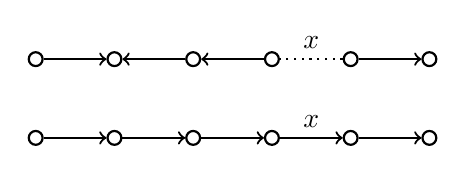
\begin{tikzpicture}
        \node[circle,draw,thick,minimum size=5pt,inner sep=0pt] (u1) at (0,0) {};
        \node[circle,draw,thick,minimum size=5pt,inner sep=0pt] (u2) at (1,0) {};
        \node[circle,draw,thick,minimum size=5pt,inner sep=0pt] (u3) at (2,0) {};
        \node[circle,draw,thick,minimum size=5pt,inner sep=0pt] (u4) at (3,0) {};
                                             
        \node[circle,draw,thick,minimum size=5pt,inner sep=0pt] (u5) at (4,0) {};
        \node[circle,draw,thick,minimum size=5pt,inner sep=0pt] (u6) at (5,0) {};

        \draw[thick,dotted,-] (u5) to node[midway,above] {$x$} (u4);
        \draw[thick,->] (u1) to (u2);
        \draw[thick,->] (u3) to (u2);
        \draw[thick,->] (u4) to (u3);
        \draw[thick,->] (u5) to (u6);

        \node[circle,draw,thick,minimum size=5pt,inner sep=0pt] (u1') at (0,-1) {};
        \node[circle,draw,thick,minimum size=5pt,inner sep=0pt] (u2') at (1,-1) {};
        \node[circle,draw,thick,minimum size=5pt,inner sep=0pt] (u3') at (2,-1) {};
        \node[circle,draw,thick,minimum size=5pt,inner sep=0pt] (u4') at (3,-1) {};
                                                                             
        \node[circle,draw,thick,minimum size=5pt,inner sep=0pt] (u5') at (4,-1) {};
        \node[circle,draw,thick,minimum size=5pt,inner sep=0pt] (u6') at (5,-1) {};

        \draw[thick,->] (u4') to node[midway,above] {$x$} (u5');
        \draw[thick,->] (u1') to (u2');
        \draw[thick,->] (u2') to (u3');
        \draw[thick,->] (u3') to (u4');
        \draw[thick,->] (u5') to (u6');
      \end{tikzpicture}

      
      \caption{Connecting two trees. The second figure shows the new graph after
        the insertion of $x$ to the position on its left.}
      \label{fig:cuckoo-insert-1}
    \end{marginfigure}

    In the figure, an arrow $u \to v$ indicates that the item corresponding to
    the edge $(u,v)$ is placed in position $u$ and its alternate location (given
    by $h_2$) is $v$. Since the two components are trees, we can direct the
    edges this way to create a DAG. Since every DAG has a sink node, there is
    some node in this graph which does not have an outgoing edge. Observe that a
    node is a sink iff there is no element in that position in the hash
    table. Thus, on inserting $x$, we could choose the position corresponding to
    $h_1(x)$, and the elements starting from the one in $h_1(x)$ will be moved
    until a sink in that directed graph is obtained. This requires $O(s)$-time
    in the worst case.
  \item If the two positions corresponding to $x$ lie in the same component,
    then the component is a tree, and adding $x$ into the hash table creates a
    single cycle in the cuckoo graph. This case is similar to the previous case
    since we can find the path to the sink in the directed version of the graph
    and move all the elements accordingly.
  \item The final case is when $x$ connects two components, one of which is a
    tree and the other contains exactly one cycle. If $h_1(x)$ belongs to the
    component containing the tree, then the insertion proceeds in the same way
    as the previous cases. The only thing to consider is when $h_1(x)$ belongs
    to the component containing the cycle. Firstly, observe that if we direct
    the edges like before, then we have directed cycle and edges directed
    towards the cycle (try to prove why this must be the case). See the figure
    on the right, for example.

    \begin{marginfigure}
      \centering
      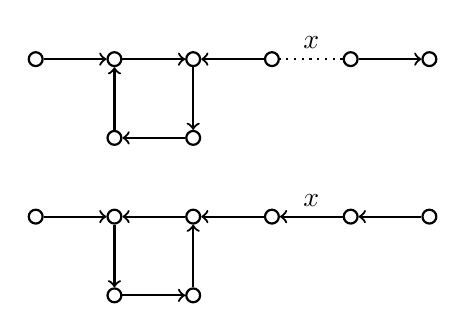
\begin{tikzpicture}
        \node[circle,draw,thick,minimum size=5pt,inner sep=0pt] (u1) at (0,0) {};
        \node[circle,draw,thick,minimum size=5pt,inner sep=0pt] (u2) at (1,0) {};
        \node[circle,draw,thick,minimum size=5pt,inner sep=0pt] (u3) at (2,0) {};
        \node[circle,draw,thick,minimum size=5pt,inner sep=0pt] (u4) at (2,-1) {};
        \node[circle,draw,thick,minimum size=5pt,inner sep=0pt] (u5) at (1,-1) {};
        \node[circle,draw,thick,minimum size=5pt,inner sep=0pt] (u6) at (3,0) {};
        \node[circle,draw,thick,minimum size=5pt,inner sep=0pt] (u7) at (4,0) {};
        \node[circle,draw,thick,minimum size=5pt,inner sep=0pt] (u8) at (5,0) {};
       
        \draw[thick,->] (u1) to (u2);
        \draw[thick,->] (u2) to (u3); \draw[thick,->] (u3) to (u4);
        \draw[thick,->] (u4) to (u5); \draw[thick,->] (u5) to (u2);
        \draw[thick,->] (u6) to (u3); \draw[thick,->] (u7) to (u8);
        \draw[thick,dotted,-] (u7) to node[midway,above] {$x$} (u6);

        \node[circle,draw,thick,minimum size=5pt,inner sep=0pt] (u1') at (0,-2) {};
        \node[circle,draw,thick,minimum size=5pt,inner sep=0pt] (u2') at (1,-2) {};
        \node[circle,draw,thick,minimum size=5pt,inner sep=0pt] (u3') at (2,-2) {};
        \node[circle,draw,thick,minimum size=5pt,inner sep=0pt] (u4') at (2,-3) {};
        \node[circle,draw,thick,minimum size=5pt,inner sep=0pt] (u5') at (1,-3) {};
        \node[circle,draw,thick,minimum size=5pt,inner sep=0pt] (u6') at (3,-2) {};
        \node[circle,draw,thick,minimum size=5pt,inner sep=0pt] (u7') at (4,-2) {};
        \node[circle,draw,thick,minimum size=5pt,inner sep=0pt] (u8') at (5,-2) {};
       
        \draw[thick,->] (u1') to (u2');
        \draw[thick,->] (u3') to (u2'); \draw[thick,->] (u4') to (u3');
        \draw[thick,->] (u5') to (u4'); \draw[thick,->] (u2') to (u5');
        \draw[thick,->] (u6') to (u3'); \draw[thick,->] (u8') to (u7');
        \draw[thick,->] (u7') to node[midway,above] {$x$} (u6');
      \end{tikzpicture}
      
      \caption{Inserting an element $x$ that connects a tree with a component
        with a single cycle. The second figure is the final connected component
        with the directions. Here $h_1(x)$ is the vertex to the left of $x$.}
      \label{fig:cuckoo-insert-2}
    \end{marginfigure}

    The insertion proceeds as follows: starting from $h_1(x)$, we will traverse
    the directed graph along the directed edges to the cycle, then traverse the
    cycle and come back to $h_1(x)$. When an edge $u\to v$ is traversed, the
    item in position $u$ is moved to the position $v$ and the direction of the
    edge changes. Once we reach back to $h_1(x)$, $x$ is moved to $h_2(x)$ which
    is in the other component (that is a cycle), and we keep moving until we
    reach a sink node like in the tree case. The each edge in the component
    containing the cycle is potentially traversed twice, and the total time is
    $O(s)$.
  \end{enumerate}
\end{proof}

We will now try to upper bound the size of connected components in the cuckoo
graph when $m$ items are inserted into a hash table of size $n$, where
$m = \tfrac{1-\epsilon}{2}n$. Since the hash functions are random, this is
equivalent to understanding the properties of the graph $G_{n,m}$, which is
uniform distribution over all graphs on $n$ vertices with $m$ edges. It turns
out that an easier graph to analyze is the Erd\"{o}-Renyi random graph $G_{n,p}$
which is the uniform distribution over graphs on $n$ vertices, where for each
pair of vertices, we add an edge with probability $p$, independently of all the
other pairs. \marginnote{You may note a similarity in the way we analyze
  $G_{n,p}$ instead of $G_{n,m}$ and approximating the balls-in-bins
  distribution using the Poisson distribution.}We will need to first show that
bounding the probability that there are no large components in $G_{n,p}$ (where
$p=m/\binom{n}{2}$) is sufficient to bound the probability that there are no
large components in $G_{n,m}$. We will assume for now that there are no
self-loops or edges in the graph sampled from $G_{n,m}$, since they cannot
increase the size of the connected components.

We will prove the following statements about the size of the connected
components in the cuckoo graph.
\begin{theorem}
  Let $G$ be a cuckoo graph with $n$ vertices and $m = \frac{1-\epsilon}{2} n$
  edges for some constant $\epsilon > 0$. Then, the following statements hold.
  \begin{enumerate}
  \item With probability $1 - 1/n$, the largest component in $G$ has size $O(\log n)$.
  \item The expected size of any connected component in $G$ is $O(1)$.
  \end{enumerate}
  \label{thm:cuckoo-cc}
\end{theorem}

Instead of proving this statement for graphs in $G_{n,m}$, we are going to prove
this for graphs in $G_{n,p}$. To that end, we will first show a connection
between the two graph distributions.

\begin{lemma}
  Let ${\cal P}$ be a any \emph{monotone graph property}. \marginnote{A monotone
    graph property is one where if $G\in {\cal P}$ and $G \subseteq G'$, then
    $G' \in {\cal P}$. For instance, connectivity is a monotone graph property
    since if $G$ is connected and we add more edges to $G$ to obtain $G'$, then
    $G'$ will also be connected.}
  Suppose that $P(n,m)$ and $P(n,p)$ are probability values defined as follows:
  \begin{align*}
    P(n,m) &= \Pr_{G\sim G_{n,m}}[G \in {\cal P}], \\
    P(n,p) &= \Pr_{G \sim G_{n,p}}[G \in {\cal P}]
  \end{align*}
  Let $p^{+} = (1+\epsilon)\frac{m}{\binom{n}{2}}$ and
  $p^- = (1-\epsilon)\frac{m}{\binom{n}{2}}$, for some constant $0 < \epsilon < 1$. Then,
  \begin{align*}
    P(n,p^-) - e^{-O(m)} < P(n,m) < P(n,p^+) + e^{-O(m)}
  \end{align*}
  \label{lem:random-graph-equiv}
\end{lemma}
\begin{proof}
  Let us first consider $P(n,p^-)$. Let $X$ be the number of edges in $G$
  sampled from $G_{n,p^-}$. Conditioned on $X=m$, the distribution of
  $G\sim G_{n,p^-}$ is identical to $G_{n,m}$. Thus, we can write the
  probability $P(n,p^-)$ as follows.
  \begin{align*}
    P(n,p^-) &= \sum_{k\geq 0} P(n,k)\cdot \Pr[X=k]
  \end{align*}
  Since ${\cal P}$ is a monotone graph property, if $k \leq k'$, then
  $P(n,k) \leq P(n,k')$. Therefore, we can split the sum as follows.
  \begin{align*}
    P(n,p^-) &\leq P(n,m) + \Pr[X > m].
  \end{align*}
  Notice that $\E[X] = p^+ \binom{n}{2}$, and it is the sum of independent
  Poisson trials. Therefore, we can apply Chernoff bounds to upper bound
  $\Pr[X>m]$.
  \begin{align*}
    \Pr[X > m] &= \Pr\left[ X \geq \frac{1}{1-\epsilon}\E[X]  \right] \leq
                 \Pr\left[ X \geq (1+\epsilon)\E[X] \right]\\
               &= \exp\left( \frac{-\epsilon^2\E[X]}{3} \right) =
                 \exp\left( \frac{-(1+\epsilon)\epsilon^2 m}{3}  \right).
  \end{align*}
  A similar calculation for $p^+$ will show the other side of the inequality in
  the lemma.
\end{proof}

Now we prove Theorem~\ref{thm:cuckoo-cc} for random graphs obtained from
$G_{n,p}$. From the lemma above this suffices, since the property of a graph
having a connected component of size at least $k$ is a monotone property.

\begin{proof}
  [Proof of Theorem~\ref{thm:cuckoo-cc}]
  In our case, we have $m = \frac{1-\epsilon}{2} n$, and we will use
  Lemma~\ref{lem:random-graph-equiv} with
  $p^+ = (1+\epsilon) \frac{m}{\binom{n}{2}} =
  \frac{(1+\epsilon)(1-\epsilon)}{n-1}$. To upper bound the size of the
  connected component, let us start by looking at a BFS starting from a fixed
  vertex $v$. The number of neighbors of $v$ in a graph in $G_{n,p^+}$ is a
  binomial random variable with parameters $n-1$ and $p^+$. For the $i^{th}$
  vertex $v_i$ in the BFS, let $N_i$ be the number of new neighbors of $v_i$ that
  are present in $G_{n,p^+}$ conditioned on the first $i-1$ vertices $v_1$,
  $v_2$, $\ldots$, $v_{i-1}$.

  The key observation here is that $N_i$ is \emph{statistically dominated} by
  the binomial random variable $B_i$ with parameters $n-1$ and $p^+$. To see
  this, notice that the random variable $N_i$ is distributed between $1$ and
  $n-i$ and each new vertex is a neighbor of $v_i$ indepenedently with
  probability $p^+$. Thus, we can say that
  $$\Pr[N_i \geq k] \leq \Pr[B_i \geq k].$$

  To bound the probability that the largest component is of size at most $s$, we
  need to upper-bound the probability of the event $\sum_{i=1}^s N_i > s$. We
  will do this by bounding the probability of the event $\sum_{i=1}^s B_i > s$
  and using the observation above.  \marginnote{ If $X$ and $Y$ are binomial
    random variables with parameters $n$ and $p$, then both $X$ and $Y$ can be
    expressed as the sum of $n$ independent Bernoulli random variables with
    parameter $p$, and hence $X+Y$ is the sum of $2n$ independent Bernoulli
    random variables with parameter $p$.  } Observe that the sum of $s$ binomial
  random variables with parameters $n-1$ and $p^+$ is another binomial random
  variable, say $B$, with parameter $s(n-1)$ and $p^+$. Also,
  $\E[B] = s(n-1)p^+ = (1-\epsilon^2) s$. Thus, we can use Chernoff bounds to
  upper bound the probability as follows.
  \begin{align*}
    \Pr\left[\sum_{i=1}^s B_i > s  \right] &= \Pr\left[ B > s \right] = \Pr\left[ B \geq \frac{\E[B]}{1-\epsilon^2}  \right]\\
    &\leq \Pr\left[ B \geq (1+\epsilon^2)\E[B] \right] \leq e^{-\epsilon^2 \E[B]/3}
  \end{align*}
  Thus, if $s \geq \frac{4\ln n}{\epsilon^2 (1-\epsilon^2)}$, we have
  $\Pr[B \geq s] \leq n^{-2}$. Thus, the probability that there is some vertex
  $v$ such that a BFS from $v$ will find a component of size more than $s$ is at
  most $1/n$.

  To prove Part (2) of the theorem, let $S$ denote the size of the connected
  component containing a fixed vertex $v$ in a graph sampled according to
  $G_{n,m}$, and let $S'$ denote the size of the connected component containing
  the vertex $v$ in a graph sampled according to $G_{n,p^+}$. From
  Lemma~\ref{lem:random-graph-equiv}, we can say that
  $Pr[S \geq s] \leq \Pr[S' \geq s] + e^{-O(m)}$. Since
  $\E[S] = \sum_{k=1}^n \Pr[S \geq k]$, we can write
  \begin{align*}
    \E[S] \leq \sum_{k=1}^n \Pr[S' \geq k] + ne^{-O(m)} = \E[S'] + ne^{-O(m)}.
  \end{align*}

  To finish the proof of Part (2), we need to show that $\E[S'] =
  O(1)$. Consider the BFS starting from $v$ that explores this connected
  component. Let $X_i$ be the number of vertices obtained in the $i^{th}$ level
  of this BFS tree. Here $X_1$ contains the vertex $v$. We can say that
  \begin{align*}
    S' &= \sum_{i \geq 1} X_i, \text{ and therefore, }\\
    \E[S'] &= \sum_{i \geq 1} \E[X_i].
  \end{align*}

  Instead of working with the random variables $X_i$, we will instead use the
  observation that the random variable correspondig to the number of new
  neighbors discovered by a vertex in a BFS is statistically dominated by a
  binomial random variable with parameters $n-1$ and $p^+$. Let $Y_i$ be the
  random variable corresponding to the number of vertices in the $i^{th}$ level
  when each vertex in the $(i-1)^{st}$ level chooses according to the binomial
  distribution.
  
  Now, for any $i \geq 2$, we can write $\E[Y_i]$ using conditional expectation
  as $\E[Y_i] = \sum_{k \geq 0} \Pr[Y_{i-1} = k]\cdot \E[Y_i ~|~ Y_{i-1} =
  k]$. We can write the conditional expection in the following manner. Suppose
  that $Z_j$ is the random variable corresponding to the number of vertices
  obtained using the binomial distribution from the vertex $j$ in the level $i-1$.
  \begin{align*}
    \E[Y_i ~|~ Y_{i-1} =k] &= \E\left[ \sum_{j=1}^{k} Z_j \right]\\
    &= k(n-1)p^+
  \end{align*}

  Thus, we can write the expectation
  \begin{align*}
    \E[Y_i] &= \sum_{k \geq 0} (n-1)p^+ k\Pr[Y_{i-1}=k]\\
    &= (n-1)p^+\E[Y_{i-1}] = ((n-1)p^+)^i = (1-\epsilon^2)^i
  \end{align*}
  Hence, $\E[S'] \leq \sum_{i\geq 1} (1-\epsilon^2)^i = O(1)$.
\end{proof}

To complete the analysis of cuckoo hashing, we need to prove one more
thing. Recall that if the connected component contains more than one cycle, then
the entire table has to be rehashed. We will now show that, with high
probability, the small connected components in the cuckoo graph are either trees
or have only one cycle.

\begin{theorem}
  Let $G$ be a cuckoo graph on $n$ vertices and $m=(1-\epsilon)n/2$ edges, for a
  constant $\epsilon > 0$. Then, with high probability, all the
  connected components of size at most $\Theta(\log n)$ are either trees or
  graphs with exactly one cycle.
  \label{thm:cuckoo-graph-unicycle}
\end{theorem}
\begin{proof}
  For proving this we will use Cayley's theorem that states that there are
  $k^{k-2}$ labelled trees on $k$ vertices. For a component of size $k$ to
  contain at least two cycles, the component must contain at least $k+1$
  edges. We will show that for $k = \Theta(\log n)$, the probability of there
  being connected components of size $k$ and containing $k+1$ edges is at most
  $1/n$.

  For a fixed set of $k$ vertices, the probability that the vertices form a
  connected component with $k+1$ edges is obtained as follows:
  \begin{itemize}
  \item Choose one among the $k^{k-2}$ labelled trees on $k$ vertices - this can
    be done in $k^{k-2}$ ways.
  \item Choose order in which these edges will be picked while sampling a graph
    - this can be done in $\binom{m}{k-1} (k-1)!$ ways.
  \item Choose the order in which the two additional edges in the component will
    be picked - $\binom{m-k+1}{2} k^4$.
  \end{itemize}
  Thus, the expression for the probability that the
  component on these fixed $k$ vertices contains more than one cycle is at most
  \begin{align*}
    k^{k-2} \binom{m}{k-1} (k-1)! \left( \frac{1}{n^2} \right)^{k-1} \binom{m-k+1}{2} k^4 \left( \frac{1}{n^2} \right)^2 \left(1 - \frac{k(n-k)}{n^2} \right)^{m-k-1}.
  \end{align*}
  Hence, the probability that there is some component of size $k$ containing more
  than two cycles is upper-bounded by the following expression.
  \begin{align*}
    &\binom{n}{k}k^{k-2} \binom{m}{k-1} (k-1)! \left( \frac{1}{n^2} \right)^{k-1} \binom{m-k+1}{2} k^4 \left( \frac{1}{n^2} \right)^2 \left(1 - \frac{k(n-k)}{n^2} \right)^{m-k-1}\\
    &\leq \frac{n^k}{k!} \frac{k^k}{k^2} \frac{m!}{(k-1)!(m-k+1)!} \frac{(m-k+1)!}{2! (m-k-1)!} (k-1)! \left(\frac{1}{n^2} \right)^{k-1} \frac{k^4}{n^4} e^{-k(n-k)(m-k-1)/n^2}\\
    &\leq \frac{e^k m^{k+1}}{2} \frac{k^2}{n^{k+2}}e^{-k(n-k)(m-k-1)/n^2}\\
    &\leq \frac{e^kk^2(1-\epsilon)^{k+1}}{2^{k+2}n^2}e^{-k(n-k)(m-k-1)/n^2}, \text{ using $m=(1-\epsilon)n/2$}\\
    &\leq \frac{k^2}{4n}(1-\epsilon)^{k+1}e^{-2nmk/n^2}e^{4k^2/n}, \text{ using $k=\Theta(\log n)$}\\
    &\leq \frac{k^2}{2n}(1-\epsilon)^{k+1}e^{-(1-\epsilon)k}\\
    &\leq \frac{1}{n^\alpha}(1-\epsilon)^{k+1}e^{\epsilon k} \leq \frac{1}{n^\alpha} e^{k(\epsilon + \ln(1-\epsilon))}
  \end{align*}

  Now, $\epsilon+\ln(1-\epsilon) = \Theta(\epsilon^2)$. Hence the probability that there is some connected component of size at most $k = O(\log n)$ that contains more than once cyle is at most $1/n^\alpha$ for a constant $\alpha > 0$.
\end{proof}

%%% Local Variables: 
%%% mode: latex
%%% TeX-master: "notes"
%%% End:
